
% Default to the notebook output style

    


% Inherit from the specified cell style.




    
\documentclass[11pt]{article}

    
    
    \usepackage[T1]{fontenc}
    % Nicer default font (+ math font) than Computer Modern for most use cases
    \usepackage{mathpazo}

    % Basic figure setup, for now with no caption control since it's done
    % automatically by Pandoc (which extracts ![](path) syntax from Markdown).
    \usepackage{graphicx}
    % We will generate all images so they have a width \maxwidth. This means
    % that they will get their normal width if they fit onto the page, but
    % are scaled down if they would overflow the margins.
    \makeatletter
    \def\maxwidth{\ifdim\Gin@nat@width>\linewidth\linewidth
    \else\Gin@nat@width\fi}
    \makeatother
    \let\Oldincludegraphics\includegraphics
    % Set max figure width to be 80% of text width, for now hardcoded.
    \renewcommand{\includegraphics}[1]{\Oldincludegraphics[width=.8\maxwidth]{#1}}
    % Ensure that by default, figures have no caption (until we provide a
    % proper Figure object with a Caption API and a way to capture that
    % in the conversion process - todo).
    \usepackage{caption}
    \DeclareCaptionLabelFormat{nolabel}{}
    \captionsetup{labelformat=nolabel}

    \usepackage{adjustbox} % Used to constrain images to a maximum size 
    \usepackage{xcolor} % Allow colors to be defined
    \usepackage{enumerate} % Needed for markdown enumerations to work
    \usepackage{geometry} % Used to adjust the document margins
    \usepackage{amsmath} % Equations
    \usepackage{amssymb} % Equations
    \usepackage{textcomp} % defines textquotesingle
    % Hack from http://tex.stackexchange.com/a/47451/13684:
    \AtBeginDocument{%
        \def\PYZsq{\textquotesingle}% Upright quotes in Pygmentized code
    }
    \usepackage{upquote} % Upright quotes for verbatim code
    \usepackage{eurosym} % defines \euro
    \usepackage[mathletters]{ucs} % Extended unicode (utf-8) support
    \usepackage[utf8x]{inputenc} % Allow utf-8 characters in the tex document
    \usepackage{fancyvrb} % verbatim replacement that allows latex
    \usepackage{grffile} % extends the file name processing of package graphics 
                         % to support a larger range 
    % The hyperref package gives us a pdf with properly built
    % internal navigation ('pdf bookmarks' for the table of contents,
    % internal cross-reference links, web links for URLs, etc.)
    \usepackage{hyperref}
    \usepackage{longtable} % longtable support required by pandoc >1.10
    \usepackage{booktabs}  % table support for pandoc > 1.12.2
    \usepackage[inline]{enumitem} % IRkernel/repr support (it uses the enumerate* environment)
    \usepackage[normalem]{ulem} % ulem is needed to support strikethroughs (\sout)
                                % normalem makes italics be italics, not underlines
    

    
    
    % Colors for the hyperref package
    \definecolor{urlcolor}{rgb}{0,.145,.698}
    \definecolor{linkcolor}{rgb}{.71,0.21,0.01}
    \definecolor{citecolor}{rgb}{.12,.54,.11}

    % ANSI colors
    \definecolor{ansi-black}{HTML}{3E424D}
    \definecolor{ansi-black-intense}{HTML}{282C36}
    \definecolor{ansi-red}{HTML}{E75C58}
    \definecolor{ansi-red-intense}{HTML}{B22B31}
    \definecolor{ansi-green}{HTML}{00A250}
    \definecolor{ansi-green-intense}{HTML}{007427}
    \definecolor{ansi-yellow}{HTML}{DDB62B}
    \definecolor{ansi-yellow-intense}{HTML}{B27D12}
    \definecolor{ansi-blue}{HTML}{208FFB}
    \definecolor{ansi-blue-intense}{HTML}{0065CA}
    \definecolor{ansi-magenta}{HTML}{D160C4}
    \definecolor{ansi-magenta-intense}{HTML}{A03196}
    \definecolor{ansi-cyan}{HTML}{60C6C8}
    \definecolor{ansi-cyan-intense}{HTML}{258F8F}
    \definecolor{ansi-white}{HTML}{C5C1B4}
    \definecolor{ansi-white-intense}{HTML}{A1A6B2}

    % commands and environments needed by pandoc snippets
    % extracted from the output of `pandoc -s`
    \providecommand{\tightlist}{%
      \setlength{\itemsep}{0pt}\setlength{\parskip}{0pt}}
    \DefineVerbatimEnvironment{Highlighting}{Verbatim}{commandchars=\\\{\}}
    % Add ',fontsize=\small' for more characters per line
    \newenvironment{Shaded}{}{}
    \newcommand{\KeywordTok}[1]{\textcolor[rgb]{0.00,0.44,0.13}{\textbf{{#1}}}}
    \newcommand{\DataTypeTok}[1]{\textcolor[rgb]{0.56,0.13,0.00}{{#1}}}
    \newcommand{\DecValTok}[1]{\textcolor[rgb]{0.25,0.63,0.44}{{#1}}}
    \newcommand{\BaseNTok}[1]{\textcolor[rgb]{0.25,0.63,0.44}{{#1}}}
    \newcommand{\FloatTok}[1]{\textcolor[rgb]{0.25,0.63,0.44}{{#1}}}
    \newcommand{\CharTok}[1]{\textcolor[rgb]{0.25,0.44,0.63}{{#1}}}
    \newcommand{\StringTok}[1]{\textcolor[rgb]{0.25,0.44,0.63}{{#1}}}
    \newcommand{\CommentTok}[1]{\textcolor[rgb]{0.38,0.63,0.69}{\textit{{#1}}}}
    \newcommand{\OtherTok}[1]{\textcolor[rgb]{0.00,0.44,0.13}{{#1}}}
    \newcommand{\AlertTok}[1]{\textcolor[rgb]{1.00,0.00,0.00}{\textbf{{#1}}}}
    \newcommand{\FunctionTok}[1]{\textcolor[rgb]{0.02,0.16,0.49}{{#1}}}
    \newcommand{\RegionMarkerTok}[1]{{#1}}
    \newcommand{\ErrorTok}[1]{\textcolor[rgb]{1.00,0.00,0.00}{\textbf{{#1}}}}
    \newcommand{\NormalTok}[1]{{#1}}
    
    % Additional commands for more recent versions of Pandoc
    \newcommand{\ConstantTok}[1]{\textcolor[rgb]{0.53,0.00,0.00}{{#1}}}
    \newcommand{\SpecialCharTok}[1]{\textcolor[rgb]{0.25,0.44,0.63}{{#1}}}
    \newcommand{\VerbatimStringTok}[1]{\textcolor[rgb]{0.25,0.44,0.63}{{#1}}}
    \newcommand{\SpecialStringTok}[1]{\textcolor[rgb]{0.73,0.40,0.53}{{#1}}}
    \newcommand{\ImportTok}[1]{{#1}}
    \newcommand{\DocumentationTok}[1]{\textcolor[rgb]{0.73,0.13,0.13}{\textit{{#1}}}}
    \newcommand{\AnnotationTok}[1]{\textcolor[rgb]{0.38,0.63,0.69}{\textbf{\textit{{#1}}}}}
    \newcommand{\CommentVarTok}[1]{\textcolor[rgb]{0.38,0.63,0.69}{\textbf{\textit{{#1}}}}}
    \newcommand{\VariableTok}[1]{\textcolor[rgb]{0.10,0.09,0.49}{{#1}}}
    \newcommand{\ControlFlowTok}[1]{\textcolor[rgb]{0.00,0.44,0.13}{\textbf{{#1}}}}
    \newcommand{\OperatorTok}[1]{\textcolor[rgb]{0.40,0.40,0.40}{{#1}}}
    \newcommand{\BuiltInTok}[1]{{#1}}
    \newcommand{\ExtensionTok}[1]{{#1}}
    \newcommand{\PreprocessorTok}[1]{\textcolor[rgb]{0.74,0.48,0.00}{{#1}}}
    \newcommand{\AttributeTok}[1]{\textcolor[rgb]{0.49,0.56,0.16}{{#1}}}
    \newcommand{\InformationTok}[1]{\textcolor[rgb]{0.38,0.63,0.69}{\textbf{\textit{{#1}}}}}
    \newcommand{\WarningTok}[1]{\textcolor[rgb]{0.38,0.63,0.69}{\textbf{\textit{{#1}}}}}
    
    
    % Define a nice break command that doesn't care if a line doesn't already
    % exist.
    \def\br{\hspace*{\fill} \\* }
    % Math Jax compatability definitions
    \def\gt{>}
    \def\lt{<}
    % Document parameters
    \title{README}
    
    
    

    % Pygments definitions
    
\makeatletter
\def\PY@reset{\let\PY@it=\relax \let\PY@bf=\relax%
    \let\PY@ul=\relax \let\PY@tc=\relax%
    \let\PY@bc=\relax \let\PY@ff=\relax}
\def\PY@tok#1{\csname PY@tok@#1\endcsname}
\def\PY@toks#1+{\ifx\relax#1\empty\else%
    \PY@tok{#1}\expandafter\PY@toks\fi}
\def\PY@do#1{\PY@bc{\PY@tc{\PY@ul{%
    \PY@it{\PY@bf{\PY@ff{#1}}}}}}}
\def\PY#1#2{\PY@reset\PY@toks#1+\relax+\PY@do{#2}}

\expandafter\def\csname PY@tok@w\endcsname{\def\PY@tc##1{\textcolor[rgb]{0.73,0.73,0.73}{##1}}}
\expandafter\def\csname PY@tok@c\endcsname{\let\PY@it=\textit\def\PY@tc##1{\textcolor[rgb]{0.25,0.50,0.50}{##1}}}
\expandafter\def\csname PY@tok@cp\endcsname{\def\PY@tc##1{\textcolor[rgb]{0.74,0.48,0.00}{##1}}}
\expandafter\def\csname PY@tok@k\endcsname{\let\PY@bf=\textbf\def\PY@tc##1{\textcolor[rgb]{0.00,0.50,0.00}{##1}}}
\expandafter\def\csname PY@tok@kp\endcsname{\def\PY@tc##1{\textcolor[rgb]{0.00,0.50,0.00}{##1}}}
\expandafter\def\csname PY@tok@kt\endcsname{\def\PY@tc##1{\textcolor[rgb]{0.69,0.00,0.25}{##1}}}
\expandafter\def\csname PY@tok@o\endcsname{\def\PY@tc##1{\textcolor[rgb]{0.40,0.40,0.40}{##1}}}
\expandafter\def\csname PY@tok@ow\endcsname{\let\PY@bf=\textbf\def\PY@tc##1{\textcolor[rgb]{0.67,0.13,1.00}{##1}}}
\expandafter\def\csname PY@tok@nb\endcsname{\def\PY@tc##1{\textcolor[rgb]{0.00,0.50,0.00}{##1}}}
\expandafter\def\csname PY@tok@nf\endcsname{\def\PY@tc##1{\textcolor[rgb]{0.00,0.00,1.00}{##1}}}
\expandafter\def\csname PY@tok@nc\endcsname{\let\PY@bf=\textbf\def\PY@tc##1{\textcolor[rgb]{0.00,0.00,1.00}{##1}}}
\expandafter\def\csname PY@tok@nn\endcsname{\let\PY@bf=\textbf\def\PY@tc##1{\textcolor[rgb]{0.00,0.00,1.00}{##1}}}
\expandafter\def\csname PY@tok@ne\endcsname{\let\PY@bf=\textbf\def\PY@tc##1{\textcolor[rgb]{0.82,0.25,0.23}{##1}}}
\expandafter\def\csname PY@tok@nv\endcsname{\def\PY@tc##1{\textcolor[rgb]{0.10,0.09,0.49}{##1}}}
\expandafter\def\csname PY@tok@no\endcsname{\def\PY@tc##1{\textcolor[rgb]{0.53,0.00,0.00}{##1}}}
\expandafter\def\csname PY@tok@nl\endcsname{\def\PY@tc##1{\textcolor[rgb]{0.63,0.63,0.00}{##1}}}
\expandafter\def\csname PY@tok@ni\endcsname{\let\PY@bf=\textbf\def\PY@tc##1{\textcolor[rgb]{0.60,0.60,0.60}{##1}}}
\expandafter\def\csname PY@tok@na\endcsname{\def\PY@tc##1{\textcolor[rgb]{0.49,0.56,0.16}{##1}}}
\expandafter\def\csname PY@tok@nt\endcsname{\let\PY@bf=\textbf\def\PY@tc##1{\textcolor[rgb]{0.00,0.50,0.00}{##1}}}
\expandafter\def\csname PY@tok@nd\endcsname{\def\PY@tc##1{\textcolor[rgb]{0.67,0.13,1.00}{##1}}}
\expandafter\def\csname PY@tok@s\endcsname{\def\PY@tc##1{\textcolor[rgb]{0.73,0.13,0.13}{##1}}}
\expandafter\def\csname PY@tok@sd\endcsname{\let\PY@it=\textit\def\PY@tc##1{\textcolor[rgb]{0.73,0.13,0.13}{##1}}}
\expandafter\def\csname PY@tok@si\endcsname{\let\PY@bf=\textbf\def\PY@tc##1{\textcolor[rgb]{0.73,0.40,0.53}{##1}}}
\expandafter\def\csname PY@tok@se\endcsname{\let\PY@bf=\textbf\def\PY@tc##1{\textcolor[rgb]{0.73,0.40,0.13}{##1}}}
\expandafter\def\csname PY@tok@sr\endcsname{\def\PY@tc##1{\textcolor[rgb]{0.73,0.40,0.53}{##1}}}
\expandafter\def\csname PY@tok@ss\endcsname{\def\PY@tc##1{\textcolor[rgb]{0.10,0.09,0.49}{##1}}}
\expandafter\def\csname PY@tok@sx\endcsname{\def\PY@tc##1{\textcolor[rgb]{0.00,0.50,0.00}{##1}}}
\expandafter\def\csname PY@tok@m\endcsname{\def\PY@tc##1{\textcolor[rgb]{0.40,0.40,0.40}{##1}}}
\expandafter\def\csname PY@tok@gh\endcsname{\let\PY@bf=\textbf\def\PY@tc##1{\textcolor[rgb]{0.00,0.00,0.50}{##1}}}
\expandafter\def\csname PY@tok@gu\endcsname{\let\PY@bf=\textbf\def\PY@tc##1{\textcolor[rgb]{0.50,0.00,0.50}{##1}}}
\expandafter\def\csname PY@tok@gd\endcsname{\def\PY@tc##1{\textcolor[rgb]{0.63,0.00,0.00}{##1}}}
\expandafter\def\csname PY@tok@gi\endcsname{\def\PY@tc##1{\textcolor[rgb]{0.00,0.63,0.00}{##1}}}
\expandafter\def\csname PY@tok@gr\endcsname{\def\PY@tc##1{\textcolor[rgb]{1.00,0.00,0.00}{##1}}}
\expandafter\def\csname PY@tok@ge\endcsname{\let\PY@it=\textit}
\expandafter\def\csname PY@tok@gs\endcsname{\let\PY@bf=\textbf}
\expandafter\def\csname PY@tok@gp\endcsname{\let\PY@bf=\textbf\def\PY@tc##1{\textcolor[rgb]{0.00,0.00,0.50}{##1}}}
\expandafter\def\csname PY@tok@go\endcsname{\def\PY@tc##1{\textcolor[rgb]{0.53,0.53,0.53}{##1}}}
\expandafter\def\csname PY@tok@gt\endcsname{\def\PY@tc##1{\textcolor[rgb]{0.00,0.27,0.87}{##1}}}
\expandafter\def\csname PY@tok@err\endcsname{\def\PY@bc##1{\setlength{\fboxsep}{0pt}\fcolorbox[rgb]{1.00,0.00,0.00}{1,1,1}{\strut ##1}}}
\expandafter\def\csname PY@tok@kc\endcsname{\let\PY@bf=\textbf\def\PY@tc##1{\textcolor[rgb]{0.00,0.50,0.00}{##1}}}
\expandafter\def\csname PY@tok@kd\endcsname{\let\PY@bf=\textbf\def\PY@tc##1{\textcolor[rgb]{0.00,0.50,0.00}{##1}}}
\expandafter\def\csname PY@tok@kn\endcsname{\let\PY@bf=\textbf\def\PY@tc##1{\textcolor[rgb]{0.00,0.50,0.00}{##1}}}
\expandafter\def\csname PY@tok@kr\endcsname{\let\PY@bf=\textbf\def\PY@tc##1{\textcolor[rgb]{0.00,0.50,0.00}{##1}}}
\expandafter\def\csname PY@tok@bp\endcsname{\def\PY@tc##1{\textcolor[rgb]{0.00,0.50,0.00}{##1}}}
\expandafter\def\csname PY@tok@fm\endcsname{\def\PY@tc##1{\textcolor[rgb]{0.00,0.00,1.00}{##1}}}
\expandafter\def\csname PY@tok@vc\endcsname{\def\PY@tc##1{\textcolor[rgb]{0.10,0.09,0.49}{##1}}}
\expandafter\def\csname PY@tok@vg\endcsname{\def\PY@tc##1{\textcolor[rgb]{0.10,0.09,0.49}{##1}}}
\expandafter\def\csname PY@tok@vi\endcsname{\def\PY@tc##1{\textcolor[rgb]{0.10,0.09,0.49}{##1}}}
\expandafter\def\csname PY@tok@vm\endcsname{\def\PY@tc##1{\textcolor[rgb]{0.10,0.09,0.49}{##1}}}
\expandafter\def\csname PY@tok@sa\endcsname{\def\PY@tc##1{\textcolor[rgb]{0.73,0.13,0.13}{##1}}}
\expandafter\def\csname PY@tok@sb\endcsname{\def\PY@tc##1{\textcolor[rgb]{0.73,0.13,0.13}{##1}}}
\expandafter\def\csname PY@tok@sc\endcsname{\def\PY@tc##1{\textcolor[rgb]{0.73,0.13,0.13}{##1}}}
\expandafter\def\csname PY@tok@dl\endcsname{\def\PY@tc##1{\textcolor[rgb]{0.73,0.13,0.13}{##1}}}
\expandafter\def\csname PY@tok@s2\endcsname{\def\PY@tc##1{\textcolor[rgb]{0.73,0.13,0.13}{##1}}}
\expandafter\def\csname PY@tok@sh\endcsname{\def\PY@tc##1{\textcolor[rgb]{0.73,0.13,0.13}{##1}}}
\expandafter\def\csname PY@tok@s1\endcsname{\def\PY@tc##1{\textcolor[rgb]{0.73,0.13,0.13}{##1}}}
\expandafter\def\csname PY@tok@mb\endcsname{\def\PY@tc##1{\textcolor[rgb]{0.40,0.40,0.40}{##1}}}
\expandafter\def\csname PY@tok@mf\endcsname{\def\PY@tc##1{\textcolor[rgb]{0.40,0.40,0.40}{##1}}}
\expandafter\def\csname PY@tok@mh\endcsname{\def\PY@tc##1{\textcolor[rgb]{0.40,0.40,0.40}{##1}}}
\expandafter\def\csname PY@tok@mi\endcsname{\def\PY@tc##1{\textcolor[rgb]{0.40,0.40,0.40}{##1}}}
\expandafter\def\csname PY@tok@il\endcsname{\def\PY@tc##1{\textcolor[rgb]{0.40,0.40,0.40}{##1}}}
\expandafter\def\csname PY@tok@mo\endcsname{\def\PY@tc##1{\textcolor[rgb]{0.40,0.40,0.40}{##1}}}
\expandafter\def\csname PY@tok@ch\endcsname{\let\PY@it=\textit\def\PY@tc##1{\textcolor[rgb]{0.25,0.50,0.50}{##1}}}
\expandafter\def\csname PY@tok@cm\endcsname{\let\PY@it=\textit\def\PY@tc##1{\textcolor[rgb]{0.25,0.50,0.50}{##1}}}
\expandafter\def\csname PY@tok@cpf\endcsname{\let\PY@it=\textit\def\PY@tc##1{\textcolor[rgb]{0.25,0.50,0.50}{##1}}}
\expandafter\def\csname PY@tok@c1\endcsname{\let\PY@it=\textit\def\PY@tc##1{\textcolor[rgb]{0.25,0.50,0.50}{##1}}}
\expandafter\def\csname PY@tok@cs\endcsname{\let\PY@it=\textit\def\PY@tc##1{\textcolor[rgb]{0.25,0.50,0.50}{##1}}}

\def\PYZbs{\char`\\}
\def\PYZus{\char`\_}
\def\PYZob{\char`\{}
\def\PYZcb{\char`\}}
\def\PYZca{\char`\^}
\def\PYZam{\char`\&}
\def\PYZlt{\char`\<}
\def\PYZgt{\char`\>}
\def\PYZsh{\char`\#}
\def\PYZpc{\char`\%}
\def\PYZdl{\char`\$}
\def\PYZhy{\char`\-}
\def\PYZsq{\char`\'}
\def\PYZdq{\char`\"}
\def\PYZti{\char`\~}
% for compatibility with earlier versions
\def\PYZat{@}
\def\PYZlb{[}
\def\PYZrb{]}
\makeatother


    % Exact colors from NB
    \definecolor{incolor}{rgb}{0.0, 0.0, 0.5}
    \definecolor{outcolor}{rgb}{0.545, 0.0, 0.0}



    
    % Prevent overflowing lines due to hard-to-break entities
    \sloppy 
    % Setup hyperref package
    \hypersetup{
      breaklinks=true,  % so long urls are correctly broken across lines
      colorlinks=true,
      urlcolor=urlcolor,
      linkcolor=linkcolor,
      citecolor=citecolor,
      }
    % Slightly bigger margins than the latex defaults
    
    \geometry{verbose,tmargin=1in,bmargin=1in,lmargin=1in,rmargin=1in}
    
    

    \begin{document}
    
    
    \maketitle
    
    

    
    \begin{Verbatim}[commandchars=\\\{\}]
{\color{incolor}In [{\color{incolor}1}]:} \PY{o}{\PYZpc{}}\PY{k}{matplotlib} inline
        \PY{k+kn}{import} \PY{n+nn}{pandas} \PY{k}{as} \PY{n+nn}{pd}
        \PY{k+kn}{import} \PY{n+nn}{numpy} \PY{k}{as} \PY{n+nn}{np}
\end{Verbatim}


    \hypertarget{this-project-is-used-for-class-2018-0507-msds-7335-machine-learning-at-smu}{%
\subsubsection{This project is used for class 2018-0507 MSDS 7335
Machine Learning at
SMU}\label{this-project-is-used-for-class-2018-0507-msds-7335-machine-learning-at-smu}}

\begin{itemize}
\tightlist
\item
  hosted on https://github.com/post2web/santander
\item
  by Ivelin Angelov
\end{itemize}

    \hypertarget{vector-representation-of-sparse-data}{%
\section{Vector Representation of sparse
data}\label{vector-representation-of-sparse-data}}

Santander Group's dataset is a good example of challenge where we have a
very sparse high dimensional dataset and before we can do supervised
machine learning we have to represent the dataset with a denser and less
dimensional representation. The competition has two datasets: -
train.csv with approx dimensions 4459x4992. The training data represents
4459 observations with 4991 features and 1 target variable. - test.csv
with approx dimensions 49342x4991. It has more than ten times the number
of observations as compared to the training data. It doesn't have a
target variable. This is what we are asked to predict by the
competition.

All features names are sanitization with random strings. There is no
information given of what they mean. From exploration, we came to the
conclusion that they represent the amount of money for different
categories that are used in the transaction with a customer. The targets
(labels) in the training dataset represent the value of transactions for
each potential customer.

    \hypertarget{data-exploration}{%
\subsection{Data exploration}\label{data-exploration}}

    \begin{Verbatim}[commandchars=\\\{\}]
{\color{incolor}In [{\color{incolor}2}]:} \PY{n}{train} \PY{o}{=} \PY{n}{pd}\PY{o}{.}\PY{n}{read\PYZus{}csv}\PY{p}{(}\PY{l+s+s1}{\PYZsq{}}\PY{l+s+s1}{data/train.csv}\PY{l+s+s1}{\PYZsq{}}\PY{p}{)}
        \PY{n}{test} \PY{o}{=} \PY{n}{pd}\PY{o}{.}\PY{n}{read\PYZus{}csv}\PY{p}{(}\PY{l+s+s1}{\PYZsq{}}\PY{l+s+s1}{data/test.csv}\PY{l+s+s1}{\PYZsq{}}\PY{p}{)}
        \PY{n+nb}{print}\PY{p}{(}\PY{l+s+s1}{\PYZsq{}}\PY{l+s+s1}{Train Dataset shape}\PY{l+s+s1}{\PYZsq{}}\PY{p}{,} \PY{n}{train}\PY{o}{.}\PY{n}{shape}\PY{p}{)}
        \PY{n+nb}{print}\PY{p}{(}\PY{l+s+s1}{\PYZsq{}}\PY{l+s+s1}{Test Dataset shape}\PY{l+s+s1}{\PYZsq{}}\PY{p}{,} \PY{n}{train}\PY{o}{.}\PY{n}{shape}\PY{p}{)}
\end{Verbatim}


    \begin{Verbatim}[commandchars=\\\{\}]
Train Dataset shape (4459, 4993)
Test Dataset shape (4459, 4993)

    \end{Verbatim}

    \hypertarget{head-of-train-dataset}{%
\subsubsection{Head of Train Dataset}\label{head-of-train-dataset}}

    \begin{Verbatim}[commandchars=\\\{\}]
{\color{incolor}In [{\color{incolor}3}]:} \PY{n}{train}\PY{o}{.}\PY{n}{head}\PY{p}{(}\PY{l+m+mi}{2}\PY{p}{)}
\end{Verbatim}


\begin{Verbatim}[commandchars=\\\{\}]
{\color{outcolor}Out[{\color{outcolor}3}]:}           ID      target  48df886f9  0deb4b6a8  34b15f335  a8cb14b00  \textbackslash{}
        0  000d6aaf2  38000000.0        0.0          0        0.0          0   
        1  000fbd867    600000.0        0.0          0        0.0          0   
        
           2f0771a37  30347e683  d08d1fbe3  6ee66e115    {\ldots}      3ecc09859  \textbackslash{}
        0          0          0          0          0    {\ldots}            0.0   
        1          0          0          0          0    {\ldots}            0.0   
        
           9281abeea  8675bec0b  3a13ed79a  f677d4d13  71b203550  137efaa80  \textbackslash{}
        0        0.0        0.0          0          0          0          0   
        1        0.0        0.0          0          0          0          0   
        
           fb36b89d9  7e293fbaf  9fc776466  
        0          0          0          0  
        1          0          0          0  
        
        [2 rows x 4993 columns]
\end{Verbatim}
            
    \hypertarget{head-of-test-dataset}{%
\subsubsection{Head of Test Dataset}\label{head-of-test-dataset}}

    \begin{Verbatim}[commandchars=\\\{\}]
{\color{incolor}In [{\color{incolor}4}]:} \PY{n}{test}\PY{o}{.}\PY{n}{head}\PY{p}{(}\PY{l+m+mi}{2}\PY{p}{)}
\end{Verbatim}


\begin{Verbatim}[commandchars=\\\{\}]
{\color{outcolor}Out[{\color{outcolor}4}]:}           ID  48df886f9  0deb4b6a8  34b15f335  a8cb14b00  2f0771a37  \textbackslash{}
        0  000137c73        0.0        0.0        0.0        0.0        0.0   
        1  00021489f        0.0        0.0        0.0        0.0        0.0   
        
           30347e683  d08d1fbe3  6ee66e115  20aa07010    {\ldots}      3ecc09859  \textbackslash{}
        0        0.0        0.0        0.0        0.0    {\ldots}            0.0   
        1        0.0        0.0        0.0        0.0    {\ldots}            0.0   
        
           9281abeea  8675bec0b  3a13ed79a  f677d4d13  71b203550  137efaa80  \textbackslash{}
        0        0.0        0.0        0.0        0.0        0.0        0.0   
        1        0.0        0.0        0.0        0.0        0.0        0.0   
        
           fb36b89d9  7e293fbaf  9fc776466  
        0        0.0        0.0        0.0  
        1        0.0        0.0        0.0  
        
        [2 rows x 4992 columns]
\end{Verbatim}
            
    \hypertarget{distribution-of-the-labesl}{%
\subsubsection{Distribution of the
labesl}\label{distribution-of-the-labesl}}

    \begin{Verbatim}[commandchars=\\\{\}]
{\color{incolor}In [{\color{incolor}5}]:} \PY{n}{train}\PY{p}{[}\PY{l+s+s1}{\PYZsq{}}\PY{l+s+s1}{target}\PY{l+s+s1}{\PYZsq{}}\PY{p}{]}\PY{o}{.}\PY{n}{plot}\PY{p}{(}\PY{n}{kind}\PY{o}{=}\PY{l+s+s1}{\PYZsq{}}\PY{l+s+s1}{box}\PY{l+s+s1}{\PYZsq{}}\PY{p}{)}
        \PY{n+nb}{print}\PY{p}{(}\PY{l+s+s1}{\PYZsq{}}\PY{l+s+s1}{The labels have minimum of }\PY{l+s+si}{\PYZpc{}d}\PY{l+s+s1}{ and maximum of }\PY{l+s+si}{\PYZpc{}d}\PY{l+s+s1}{\PYZsq{}} \PY{o}{\PYZpc{}} \PY{p}{(}\PY{n}{train}\PY{p}{[}\PY{l+s+s1}{\PYZsq{}}\PY{l+s+s1}{target}\PY{l+s+s1}{\PYZsq{}}\PY{p}{]}\PY{o}{.}\PY{n}{min}\PY{p}{(}\PY{p}{)}\PY{p}{,} \PY{n}{train}\PY{p}{[}\PY{l+s+s1}{\PYZsq{}}\PY{l+s+s1}{target}\PY{l+s+s1}{\PYZsq{}}\PY{p}{]}\PY{o}{.}\PY{n}{max}\PY{p}{(}\PY{p}{)}\PY{p}{)}\PY{p}{)}
\end{Verbatim}


    \begin{Verbatim}[commandchars=\\\{\}]
The labels have minimum of 30000 and maximum of 40000000

    \end{Verbatim}

    \begin{center}
    \adjustimage{max size={0.9\linewidth}{0.9\paperheight}}{output_10_1.png}
    \end{center}
    { \hspace*{\fill} \\}
    
    \hypertarget{features-exploration}{%
\subsection{Features exploration}\label{features-exploration}}

Most of the values in the two datasets are zeros and zeros most probably
represent missing value for the amount in a certain category.

    \begin{Verbatim}[commandchars=\\\{\}]
{\color{incolor}In [{\color{incolor}6}]:} \PY{n}{features} \PY{o}{=} \PY{n}{train}\PY{o}{.}\PY{n}{iloc}\PY{p}{[}\PY{p}{:}\PY{p}{,}\PY{l+m+mi}{2}\PY{p}{:}\PY{p}{]}\PY{o}{.}\PY{n}{astype}\PY{p}{(}\PY{n}{np}\PY{o}{.}\PY{n}{int32}\PY{p}{)}\PY{c+c1}{\PYZsh{}.append(test)}
\end{Verbatim}


    \hypertarget{percent-missing-values}{%
\subsubsection{Percent missing values}\label{percent-missing-values}}

    \begin{Verbatim}[commandchars=\\\{\}]
{\color{incolor}In [{\color{incolor}7}]:} \PY{n}{percent\PYZus{}zeros} \PY{o}{=} \PY{p}{(}\PY{n}{features}\PY{o}{==}\PY{l+m+mi}{0}\PY{p}{)}\PY{o}{.}\PY{n}{sum}\PY{p}{(}\PY{n}{axis}\PY{o}{=}\PY{l+m+mi}{1}\PY{p}{)}\PY{o}{.}\PY{n}{mean}\PY{p}{(}\PY{p}{)} \PY{o}{/} \PY{n}{features}\PY{o}{.}\PY{n}{shape}\PY{p}{[}\PY{l+m+mi}{1}\PY{p}{]} \PY{o}{*} \PY{l+m+mi}{100}
        \PY{n+nb}{print}\PY{p}{(}\PY{n}{percent\PYZus{}zeros}\PY{p}{,} \PY{l+s+s1}{\PYZsq{}}\PY{l+s+s1}{percent of the features are zeros (missing values)}\PY{l+s+s1}{\PYZsq{}}\PY{p}{)}
\end{Verbatim}


    \begin{Verbatim}[commandchars=\\\{\}]
96.85413111171313 percent of the features are zeros (missing values)

    \end{Verbatim}

    \hypertarget{distribution}{%
\subsection{Distribution}\label{distribution}}

The distribution shows mostly zeros, two negative values, and some
transaction amount values.

    \begin{Verbatim}[commandchars=\\\{\}]
{\color{incolor}In [{\color{incolor}8}]:} \PY{n}{values\PYZus{}vector} \PY{o}{=} \PY{n}{features}\PY{o}{.}\PY{n}{values}\PY{o}{.}\PY{n}{flatten}\PY{p}{(}\PY{p}{)}
        \PY{n}{values\PYZus{}vector} \PY{o}{=} \PY{n}{values\PYZus{}vector}\PY{p}{[}\PY{n}{values\PYZus{}vector}\PY{o}{!=}\PY{l+m+mi}{0}\PY{p}{]}
        \PY{n}{pd}\PY{o}{.}\PY{n}{DataFrame}\PY{p}{(}\PY{n}{values\PYZus{}vector}\PY{p}{)}\PY{o}{.}\PY{n}{plot}\PY{p}{(}\PY{n}{kind}\PY{o}{=}\PY{l+s+s1}{\PYZsq{}}\PY{l+s+s1}{box}\PY{l+s+s1}{\PYZsq{}}\PY{p}{)}
        \PY{n+nb}{print}\PY{p}{(}\PY{l+s+s1}{\PYZsq{}}\PY{l+s+s1}{The labels have minimum of }\PY{l+s+si}{\PYZpc{}d}\PY{l+s+s1}{ and maximum of }\PY{l+s+si}{\PYZpc{}d}\PY{l+s+s1}{\PYZsq{}} \PY{o}{\PYZpc{}} \PY{p}{(}\PY{n}{values\PYZus{}vector}\PY{o}{.}\PY{n}{min}\PY{p}{(}\PY{p}{)}\PY{p}{,} \PY{n}{values\PYZus{}vector}\PY{o}{.}\PY{n}{max}\PY{p}{(}\PY{p}{)}\PY{p}{)}\PY{p}{)}
\end{Verbatim}


    \begin{Verbatim}[commandchars=\\\{\}]
The labels have minimum of -2147483648 and maximum of 960000000

    \end{Verbatim}

    \begin{center}
    \adjustimage{max size={0.9\linewidth}{0.9\paperheight}}{output_16_1.png}
    \end{center}
    { \hspace*{\fill} \\}
    
    \hypertarget{distribution-of-the-positive-values}{%
\subsubsection{Distribution of the positive
values}\label{distribution-of-the-positive-values}}

    \begin{Verbatim}[commandchars=\\\{\}]
{\color{incolor}In [{\color{incolor}9}]:} \PY{n}{values\PYZus{}vector} \PY{o}{=} \PY{n}{features}\PY{o}{.}\PY{n}{values}\PY{o}{.}\PY{n}{flatten}\PY{p}{(}\PY{p}{)}
        \PY{n}{values\PYZus{}vector} \PY{o}{=} \PY{n}{values\PYZus{}vector}\PY{p}{[}\PY{n}{values\PYZus{}vector}\PY{o}{\PYZgt{}}\PY{l+m+mi}{0}\PY{p}{]}
        \PY{n}{pd}\PY{o}{.}\PY{n}{DataFrame}\PY{p}{(}\PY{n}{values\PYZus{}vector}\PY{p}{)}\PY{o}{.}\PY{n}{plot}\PY{p}{(}\PY{n}{kind}\PY{o}{=}\PY{l+s+s1}{\PYZsq{}}\PY{l+s+s1}{box}\PY{l+s+s1}{\PYZsq{}}\PY{p}{)}
        \PY{n+nb}{print}\PY{p}{(}\PY{l+s+s1}{\PYZsq{}}\PY{l+s+s1}{The labels have minimum of }\PY{l+s+si}{\PYZpc{}d}\PY{l+s+s1}{ and maximum of }\PY{l+s+si}{\PYZpc{}d}\PY{l+s+s1}{\PYZsq{}} \PY{o}{\PYZpc{}} \PY{p}{(}\PY{n}{values\PYZus{}vector}\PY{o}{.}\PY{n}{min}\PY{p}{(}\PY{p}{)}\PY{p}{,} \PY{n}{values\PYZus{}vector}\PY{o}{.}\PY{n}{max}\PY{p}{(}\PY{p}{)}\PY{p}{)}\PY{p}{)}
\end{Verbatim}


    \begin{Verbatim}[commandchars=\\\{\}]
The labels have minimum of 52 and maximum of 960000000

    \end{Verbatim}

    \begin{center}
    \adjustimage{max size={0.9\linewidth}{0.9\paperheight}}{output_18_1.png}
    \end{center}
    { \hspace*{\fill} \\}
    
    \hypertarget{feature-selection}{%
\subsection{Feature Selection}\label{feature-selection}}

Top 1000 features are selected based on a ranking of a random forest
model, where 1000 is a hyperparameter that could be optimized. This step
could also be skipped or executed after the preprocessing step

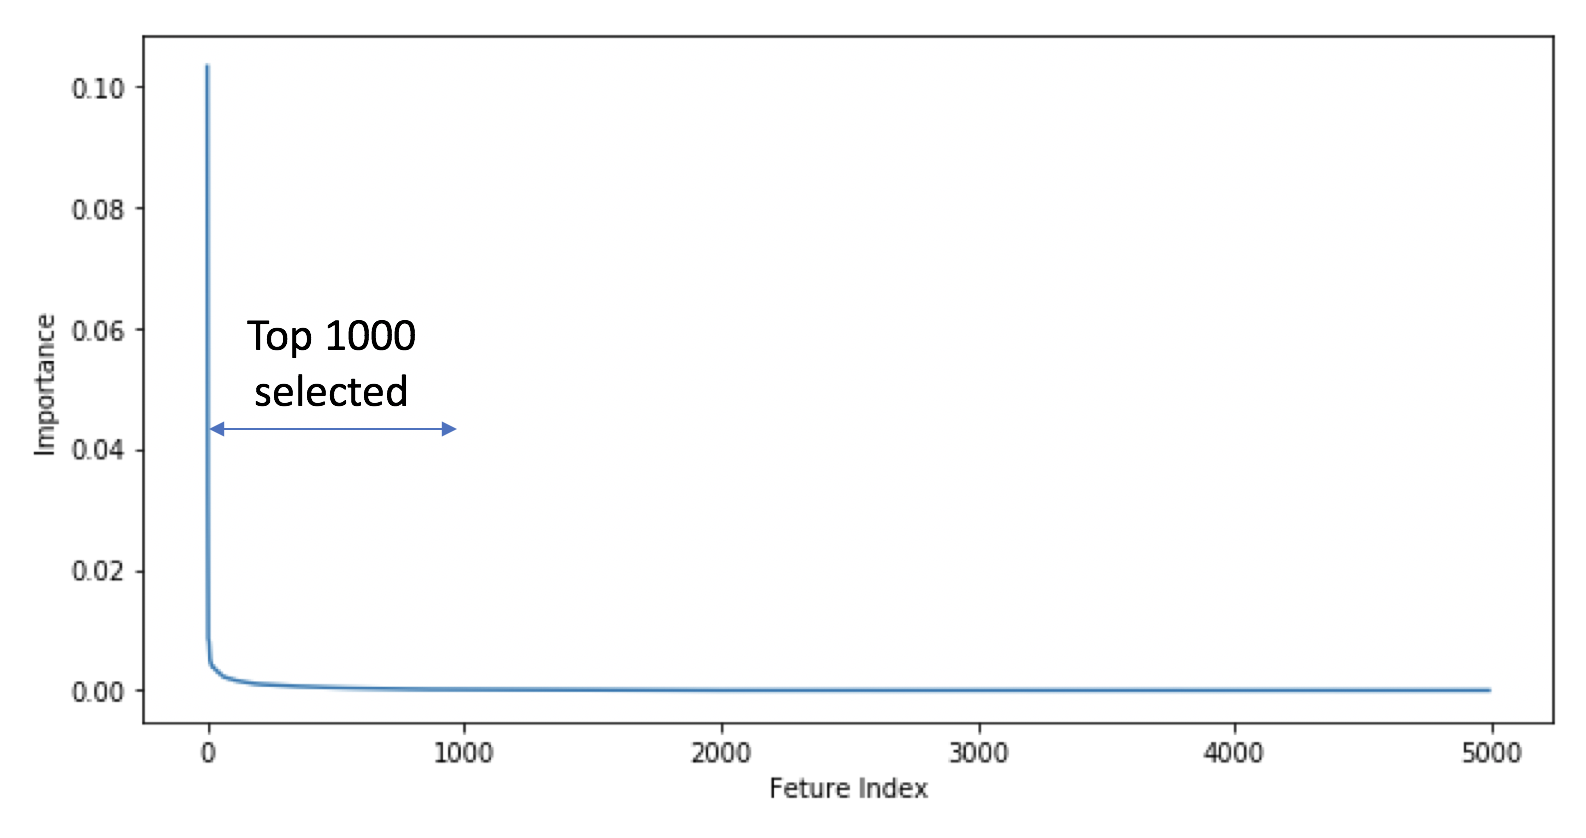
\includegraphics{images/3.png}

    \hypertarget{features-preprocessing}{%
\subsubsection{Features preprocessing}\label{features-preprocessing}}

To make the distribution less skewed, I first remove the negative values
(only two values) and log all features.

    \begin{Verbatim}[commandchars=\\\{\}]
{\color{incolor}In [{\color{incolor}23}]:} \PY{n}{preprocessed\PYZus{}features} \PY{o}{=} \PY{n}{features}\PY{o}{.}\PY{n}{copy}\PY{p}{(}\PY{p}{)}
         \PY{n}{preprocessed\PYZus{}features}\PY{p}{[}\PY{n}{preprocessed\PYZus{}features}\PY{o}{.}\PY{n}{values}\PY{o}{\PYZlt{}}\PY{l+m+mi}{0}\PY{p}{]} \PY{o}{=} \PY{l+m+mf}{0.}
         \PY{n}{preprocessed\PYZus{}features} \PY{o}{=} \PY{n}{np}\PY{o}{.}\PY{n}{log}\PY{p}{(}\PY{n}{preprocessed\PYZus{}features}\PY{o}{+}\PY{l+m+mi}{1}\PY{p}{)}
         \PY{n}{values\PYZus{}vector} \PY{o}{=} \PY{n}{preprocessed\PYZus{}features}\PY{o}{.}\PY{n}{values}\PY{o}{.}\PY{n}{flatten}\PY{p}{(}\PY{p}{)}
         \PY{k}{assert} \PY{n}{preprocessed\PYZus{}features}\PY{o}{.}\PY{n}{min}\PY{p}{(}\PY{p}{)}\PY{o}{.}\PY{n}{min}\PY{p}{(}\PY{p}{)} \PY{o}{\PYZgt{}}\PY{o}{=} \PY{l+m+mf}{0.}
         \PY{n}{pd}\PY{o}{.}\PY{n}{Series}\PY{p}{(}\PY{n}{values\PYZus{}vector}\PY{p}{)}\PY{o}{.}\PY{n}{plot}\PY{p}{(}\PY{n}{kind}\PY{o}{=}\PY{l+s+s1}{\PYZsq{}}\PY{l+s+s1}{box}\PY{l+s+s1}{\PYZsq{}}\PY{p}{)}
\end{Verbatim}


\begin{Verbatim}[commandchars=\\\{\}]
{\color{outcolor}Out[{\color{outcolor}23}]:} <matplotlib.axes.\_subplots.AxesSubplot at 0x1227600b8>
\end{Verbatim}
            
    \begin{center}
    \adjustimage{max size={0.9\linewidth}{0.9\paperheight}}{output_21_1.png}
    \end{center}
    { \hspace*{\fill} \\}
    
    To center the data around zeros I first create a new feature
representing flags for the missing values (zeros) and remove the median
from the data.

    \begin{Verbatim}[commandchars=\\\{\}]
{\color{incolor}In [{\color{incolor}24}]:} \PY{n}{zero\PYZus{}flags} \PY{o}{=} \PY{n}{preprocessed\PYZus{}features} \PY{o}{==} \PY{l+m+mf}{0.}
         \PY{n}{zero\PYZus{}flags}\PY{o}{.}\PY{n}{columns} \PY{o}{=} \PY{p}{[}\PY{n}{c}\PY{o}{+}\PY{l+s+s1}{\PYZsq{}}\PY{l+s+s1}{\PYZus{}flag}\PY{l+s+s1}{\PYZsq{}} \PY{k}{for} \PY{n}{c} \PY{o+ow}{in} \PY{n}{zero\PYZus{}flags}\PY{o}{.}\PY{n}{columns}\PY{p}{]}
         \PY{n}{values\PYZus{}vector} \PY{o}{=} \PY{n}{preprocessed\PYZus{}features}\PY{o}{.}\PY{n}{values}\PY{o}{.}\PY{n}{flatten}\PY{p}{(}\PY{p}{)}
         \PY{n}{data\PYZus{}center} \PY{o}{=} \PY{n}{np}\PY{o}{.}\PY{n}{median}\PY{p}{(}\PY{n}{values\PYZus{}vector}\PY{p}{[}\PY{n}{values\PYZus{}vector}\PY{o}{\PYZgt{}}\PY{l+m+mi}{0}\PY{p}{]}\PY{p}{)}
         
         \PY{n}{preprocessed\PYZus{}features}\PY{p}{[}\PY{o}{\PYZti{}}\PY{n}{zero\PYZus{}flags}\PY{p}{]} \PY{o}{=} \PY{n}{preprocessed\PYZus{}features}\PY{p}{[}\PY{o}{\PYZti{}}\PY{n}{zero\PYZus{}flags}\PY{p}{]} \PY{o}{\PYZhy{}} \PY{n}{data\PYZus{}center}
         \PY{n}{values\PYZus{}vector} \PY{o}{=} \PY{n}{preprocessed\PYZus{}features}\PY{o}{.}\PY{n}{values}\PY{o}{.}\PY{n}{flatten}\PY{p}{(}\PY{p}{)}
         \PY{n}{pd}\PY{o}{.}\PY{n}{DataFrame}\PY{p}{(}\PY{n}{values\PYZus{}vector}\PY{p}{)}\PY{o}{.}\PY{n}{plot}\PY{p}{(}\PY{n}{kind}\PY{o}{=}\PY{l+s+s1}{\PYZsq{}}\PY{l+s+s1}{box}\PY{l+s+s1}{\PYZsq{}}\PY{p}{)}
         
         \PY{n}{preprocessed\PYZus{}features} \PY{o}{=} \PY{n}{pd}\PY{o}{.}\PY{n}{concat}\PY{p}{(}\PY{p}{[}\PY{n}{preprocessed\PYZus{}features}\PY{p}{,} \PY{n}{zero\PYZus{}flags}\PY{p}{]}\PY{p}{,} \PY{n}{axis}\PY{o}{=}\PY{l+m+mi}{1}\PY{p}{)}
\end{Verbatim}


\begin{Verbatim}[commandchars=\\\{\}]
{\color{outcolor}Out[{\color{outcolor}24}]:} <matplotlib.axes.\_subplots.AxesSubplot at 0x12b828cf8>
\end{Verbatim}
            
    \begin{center}
    \adjustimage{max size={0.9\linewidth}{0.9\paperheight}}{output_23_1.png}
    \end{center}
    { \hspace*{\fill} \\}
    
    \hypertarget{dimensionality-reduction}{%
\subsection{Dimensionality reduction}\label{dimensionality-reduction}}

The data is now approximately normally distributed but because for every
feature I create a new ``missing flag'' it becomes even more sparse and
wide.

Two forms of dimensionality reduction are applied and compared - PCA and
Autoencoder. LDA is not considered here, because the testing dataset is
more than ten times larger than the training and it will be of great
value if included in the dimensionality reduction process.

    \hypertarget{measure-of-information-loss}{%
\subsubsection{Measure of information
loss}\label{measure-of-information-loss}}

To get some form of unsupervised performance measurements, compare the
MSE of the reconstruction of PCA and Autoencoder. The reconstruction MSE
for the Autoencoder doesn't seem to be affected by the number of
dimensions. It seems all values could fit in 2 dimensions with about the
same efficiency as they would in 128 dimensions. This is a red flag for
the Autoencoder and it could mean that even with a lot of hyperparameter
searching, I didn't achieve good training.
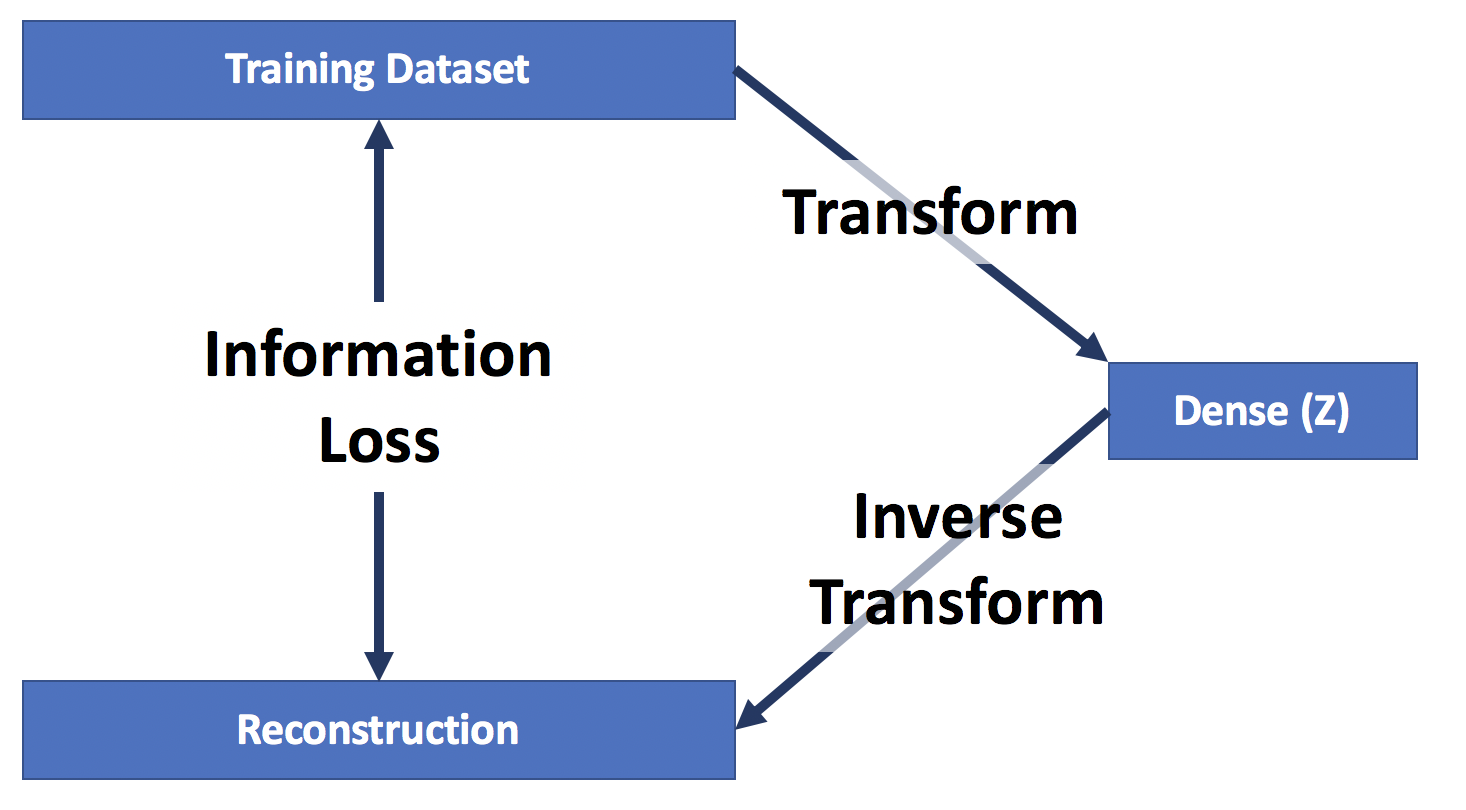
\includegraphics{images/1.png}

    \hypertarget{recreating-the-analysis}{%
\section{Recreating the analysis}\label{recreating-the-analysis}}

    \hypertarget{download-raw-data-files}{%
\subsection{Download raw data files}\label{download-raw-data-files}}

Login to Kaggle and download the data files from ``Santander Value
Prediction Challenge'':
\href{https://www.kaggle.com/c/santander-value-prediction-challenge/download/train.csv}{train.csv},
\href{https://www.kaggle.com/c/santander-value-prediction-challenge/download/test.csv}{test.csv}.
Place the files in the data folder in the root of the project.

    \hypertarget{all-steps-of-the-ml-pipeline-are-implemented-in-jupyter-notebooks.}{%
\subsection{All steps of the ML pipeline are implemented in Jupyter
notebooks.}\label{all-steps-of-the-ml-pipeline-are-implemented-in-jupyter-notebooks.}}

There are extra details and hyperparameters inside every notebook

    \hypertarget{preprocess}{%
\subsubsection{Preprocess}\label{preprocess}}

\begin{itemize}
\tightlist
\item
  This process is executed in a preprocessing notebook: preprocess.ipynb
\end{itemize}

It will apply the preprocessing logic and will save the result to
\texttt{data/train\_transformed.h5} and
\texttt{data/test\_transformed.h5}.

    \hypertarget{feature-importance}{%
\subsubsection{Feature Importance}\label{feature-importance}}

\begin{itemize}
\tightlist
\item
  This process is executed in a preprocessing notebook:
  feature\_importance.ipynb
\end{itemize}

It will rank the features and save the ranking as to
\texttt{data/importance.h5}.

    \hypertarget{dimentionality-reduction}{%
\subsubsection{Dimentionality
reduction}\label{dimentionality-reduction}}

PCA and Autoencoder are applied to the training dataset. Both training
and testing datasets are used for ``trained'' with the testing dataset.
A validation subset is used to measure unsupervised performance and
early stopping.

\begin{itemize}
\tightlist
\item
  PCA is implemented with sklean in \texttt{run\_pca.ipynb}. After
  executing the notebook, folder \texttt{pca\_result} will be populated
  with files representing encoded the training dataset for number
  different number of dimensions and validation reconstructions for
  unsupervised comparison.
\item
  Autoencoder is implemented with tensorflow in \texttt{run\_ed.ipynb},
  \texttt{ed.py}, \texttt{export\_ed.py}. After executing the notebook,
  folder \texttt{ed\_model\_dirs} will be populated with files
  representing encoded the training dataset for number different number
  of dimensions, validation reconstructions for unsupervised comparison
  and checkpoints for the tensorflow encoder-decoder models. The
  execution of the Autoencoder takes multiple hours with a fast GPU.
\end{itemize}

\hypertarget{dimentionality-reduction-unsupervied-result}{%
\paragraph{Dimentionality reduction unsupervied
result}\label{dimentionality-reduction-unsupervied-result}}

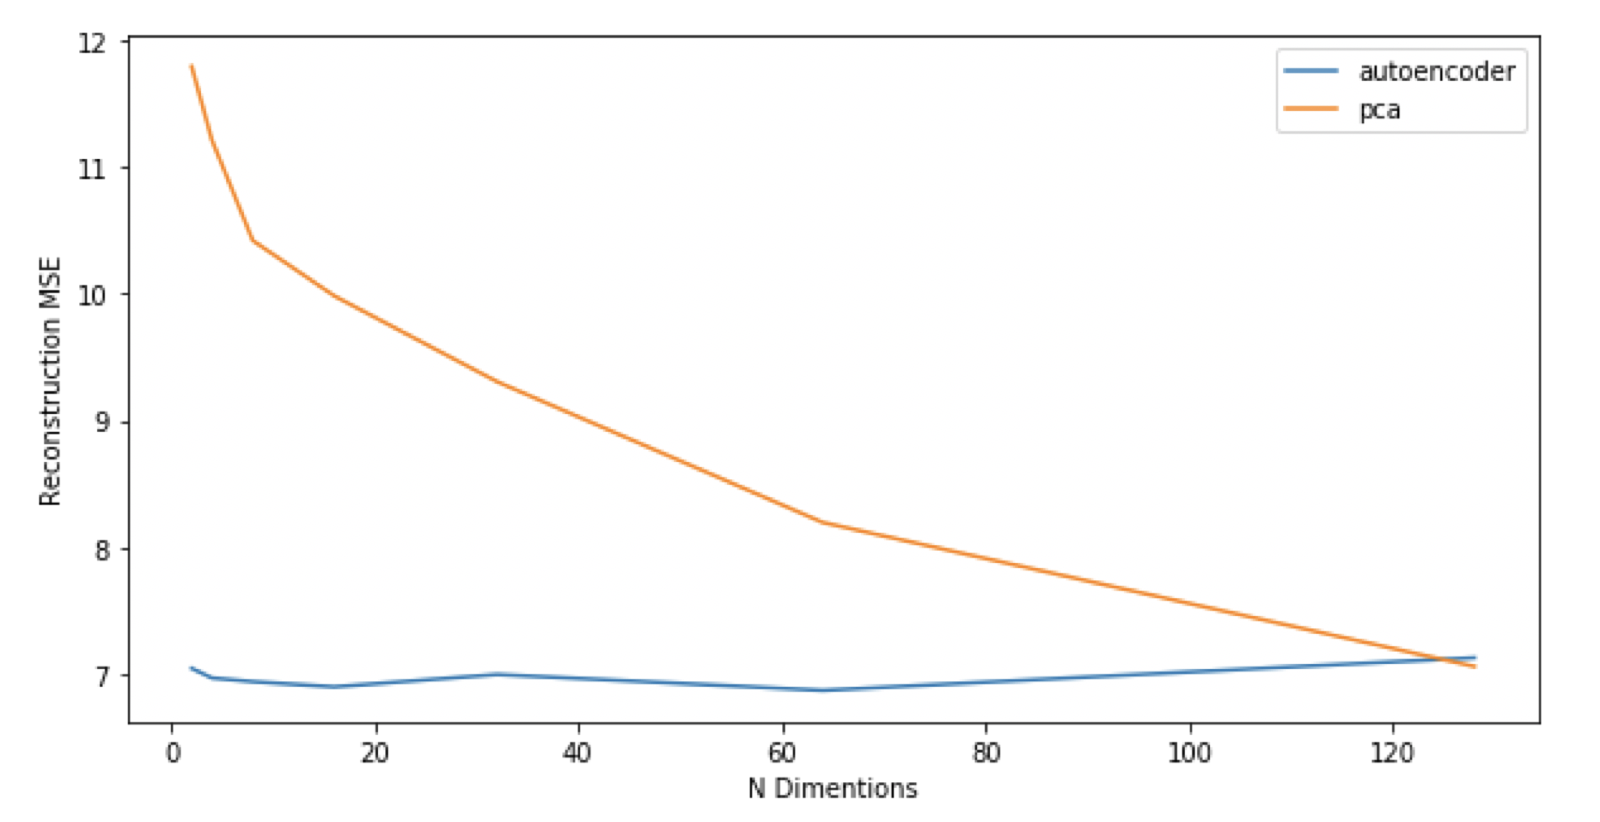
\includegraphics{images/2.png}

    \hypertarget{supervised-training}{%
\subsubsection{Supervised training}\label{supervised-training}}

After the two different dimensionality reduction methods are executed,
for every method and every number of dimensions we can apply three
different supervised regression methods: Linear Regression, Random
Forest, and Neural Network

\begin{itemize}
\tightlist
\item
  Linear Regression, Random Forest is implemented in a notebook:
  \texttt{ll\_rf.ipynb} with sklern.
\item
  Neural Network is implemented with tensorflow in notebook
  \texttt{nn.ipynb}, \texttt{nn.py} and \texttt{nn\_export.py}. The
  execution of the Neural Network takes multiple hours with a fast GPU.
\end{itemize}

    \hypertarget{linear-regression-result}{%
\paragraph{Linear Regression result}\label{linear-regression-result}}

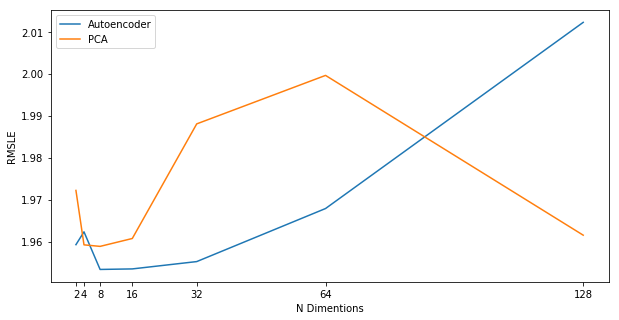
\includegraphics{images/lr.png}

    \hypertarget{random-forest-regression-result}{%
\paragraph{Random Forest Regression
result}\label{random-forest-regression-result}}

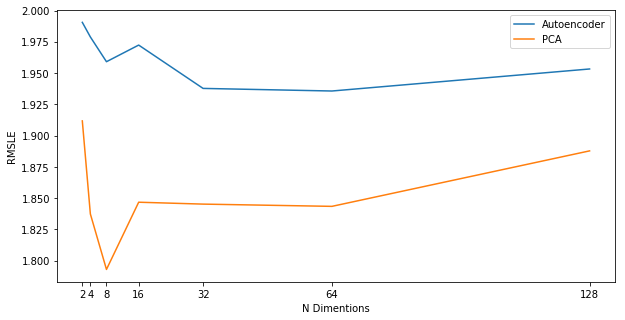
\includegraphics{images/rf.png}

    \hypertarget{neural-network-regression-result}{%
\paragraph{Neural Network Regression
result}\label{neural-network-regression-result}}

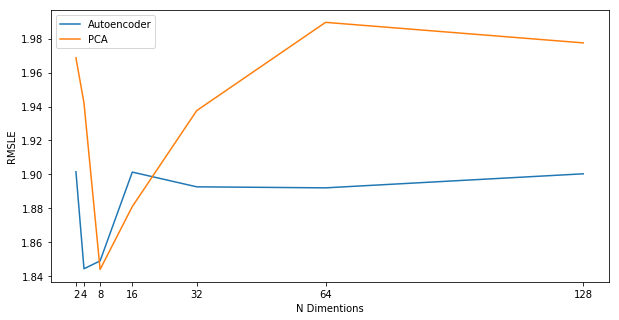
\includegraphics{images/nn.png}


    % Add a bibliography block to the postdoc
    
    
    
    \end{document}
